% Chapter 8
\chapter{Analysis with XAI Methods}
\label{ch:xai}

The scores of \cref{ch:repro,ch:gap} show that the model is weak, but not why. This chapter addresses RQ4. It uses four methods that look inside the trained model. All four methods use saved checkpoints, so they need no new training. They ran on the A10 machine.

\section{Layer-wise MSE}
\label{sec:xai-layer}

\textbf{Method.} The script \code{layer_mse.py} runs the stage 1 validation data (16 sequences, 32,768 tokens) through the teacher. Each Lizard layer gets the input of the teacher layer, as in stage 1. The script computes $1000 \times$ MSE for each layer and each head. The sum over the layers gives the stored stage 1 loss again: exactly for the float32 checkpoints, and within 0.1--0.2\% for the bf16 checkpoints. The output of the teacher grows with the depth. Thus the script also gives the \emph{relative} MSE, the MSE divided by the mean square of the teacher output.

\begin{figure}[ht]
\centering
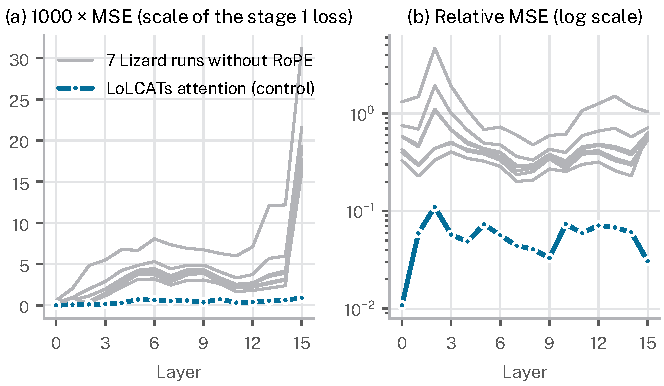
\includegraphics[width=\linewidth]{xai_layer_mse}
\caption[Layer-wise MSE of all Lizard stage 1 runs and the LoLCATs control]{Layer-wise MSE of seven Lizard stage 1 runs (gray) and the LoLCATs control (blue). (a)~$1000 \times$ MSE, the scale of the stage 1 loss. (b)~The MSE divided by the mean square of the teacher output, on a log scale. The control has a lower error in every layer. Data: the JSON files of \enquote{XAI: layer-wise MSE} in the project notes.}
\label{fig:layer-mse}
\end{figure}

\textbf{Findings.} \Cref{fig:layer-mse} shows the result.
\begin{itemize}
\item The MSE is small in the first layers and grows with the depth, as in Figure~14 of the LoLCATs paper. Layer 15 alone gives 24--31\% of the stage 1 loss.
\item Two heads of layer 15, heads 14 and 23, give approximately 20\% of the loss in every Lizard checkpoint.
\item Even with the best recipe, the error has 24--56\% of the power of the teacher output in each layer. With the recipe of the paper in bf16, ten layers have a relative MSE above 1. There, an output of zero would be closer to the teacher.
\item The recipes have the same order in all 16 layers. The difference between them is largest in the first and the last layers.
\item The LoLCATs control has a lower MSE in every layer, against every Lizard checkpoint, by a factor of at least 3.0. Its error has only 1.1--11.0\% of the power of the teacher output.
\item Heads 14 and 23 of layer 15 are not hard for the control. They give 1.9\% of its loss. Thus the teacher heads are not the problem. The Lizard layer is.
\item Layer 0 has the largest ratio between Lizard and the control (30--121 times). This agrees with the control experiment: its window has RoPE and gives the local attention of layer 0.
\end{itemize}

\section{Sample attention weights}
\label{sec:xai-weights}

\textbf{Method.} The script \code{attention_weights.py} computes the full weight matrix of each head for one sample of 1,024 tokens. For Lizard, the matrix is the gated weights plus $\alpha$ times the window weights. A check multiplies the weights with the values and gets the output of the layer again. The script compares each Lizard row with the teacher row. It uses the total variation (TV) distance after it divides the Lizard row by its sum. It also measures the weight outside the window and the weight on the first key. Plots like Figures 18--21 of the LoLCATs paper show the last 32 queries against the first 32 and the last 32 keys.

\begin{figure}[ht]
\centering
\includegraphics[width=0.94\linewidth]{xai-sample-attention-weight/trained_heads0-3_head0}
\caption[Attention weights of head 0 in five layers]{Attention weights of head 0 in five layers. The first row is the teacher. The other rows are three Lizard checkpoints. Each panel shows the last 32 queries against the first 32 keys (left of the dashed line) and the last 32 keys. The teacher has a sharp local pattern in layer 0. All Lizard checkpoints lose it. Source: project notes, \enquote{XAI: sample attention weights}.}
\label{fig:weights}
\end{figure}

\textbf{Findings.}
\begin{itemize}
\item The trained checkpoints reproduce a large part of the teacher weights. Their mean TV distance is 0.31--0.33. The start weights have 0.71.
\item The more local a teacher head is, the worse Lizard matches it. The correlation between the TV distance and the teacher weight outside the window is between $-0.75$ and $-0.78$. Heads with less than 30\% of their weight outside the window have a mean TV distance of 0.56. Heads with more than 70\% have 0.21--0.25.
\item Lizard gives all heads of a layer almost the same long-range share. Inside a layer, the teacher share outside the window has a standard deviation of 0.126 over the heads. For Lizard, it is only 0.034--0.048.
\item Layer 15, head 14 is a local head in the teacher. The teacher puts only 8.7\% of its weight outside the window. Lizard puts 50--53\% there. Its large MSE (\cref{sec:xai-layer}) comes from too much weight far away in Lizard.
\item Layer 0 is the worst layer (TV distance 0.49--0.60). Its head 2 attends to the previous token in the teacher. In all trained checkpoints, this head is almost empty (\cref{fig:weights}). The output of layer 0 is small, so the MSE hardly shows this error.
\end{itemize}

\section{MSE by token position}
\label{sec:xai-position}

\textbf{Method.} The script \code{position_mse.py} splits the query positions into three buckets: 0--127, 128--511 and 512--2047. In the first bucket, all keys are inside the window, as in almost every PIQA and ARC-Easy prompt. The script computes the relative MSE for each layer and bucket. A rank test then compares the error of each bucket with PIQA and ARC-Easy over the checkpoints.

\textbf{Findings.}
\begin{itemize}
\item The LoLCATs control computes the teacher attention at positions 0--127. Its relative MSE there is $8.4 \times 10^{-6}$ to $4.4 \times 10^{-5}$, the size of bf16 rounding.
\item Lizard misses 35--63\% of the teacher output at the same positions (relative MSE 0.351--0.629 over 8 checkpoints). This is more than 20,000 times the value of the control.
\item Layers 2 and 3 have the largest error at short positions. Layer 2 has the largest value in all 8 checkpoints (0.64--1.17).
\item The error at positions 0--127 does not predict PIQA or ARC-Easy over the Lizard checkpoints. The rank correlations are not significant. Thus this error alone cannot rank the stage 1 runs either.
\end{itemize}

The left panel of \cref{fig:position-heatmap} (\cref{ch:rope}) shows this measure for the first Lizard model.

\section{Branch decomposition}
\label{sec:xai-branch}

\textbf{Method.} The script \code{branch_fit.py} asks which branch limits the fit. For each head and each bucket, it fits the teacher output $\vy$ with a weighted sum of candidate outputs by least squares. It reports the remaining error divided by $\|\vy\|^2$. The candidates are:
\begin{itemize}
\item G: the trained gated branch,
\item W: the trained window branch, without RoPE and with the sinks,
\item WR: an oracle window that uses the teacher scores with RoPE over the same 128 keys, without sinks and without trained parameters.
\end{itemize}
The script fits every combination, for example G+W or G+WR. It also reports the error of the trained output. At positions 0--127, WR is the teacher attention, so its error must be only rounding. This is the check of the method: WR gives $1.3 \times 10^{-5}$ in bf16.

\begin{table}[ht]
\centering
\small
\caption[Results of the branch decomposition]{Results of the branch decomposition for the eight Lizard stage 1 checkpoints without RoPE (project notes, \enquote{XAI: branch decomposition}). Values are remaining errors divided by $\|\vy\|^2$.}
\label{tab:branch-fit}
\begin{tabularx}{\linewidth}{@{}LL@{}}
\toprule
Comparison & Result \\
\midrule
W alone, positions 0--127, best weight for each head & 0.394--0.458. The window without RoPE explains only approximately 60\% of the teacher output. \\
G+W against W, positions 0--127 & 0.78--0.81 $\times$. The gated branch helps only a little inside the window. \\
G+WR against WR alone, positions 512--2047 & 0.40--0.58 $\times$. Outside the window, the gated branch gives a large part of the output. \\
G+WR against G+W, all positions & 1.9--2.1 times less error. A window with RoPE would halve the error. \\
Heads 14 and 23 of layer 15, WR alone & 0.017 and 0.134--0.136, against 0.57--0.62 and 0.90--0.94 for the trained output \\
Best weight of G in the G+W fit & Median 0.55--0.81, not 1. The gated branch has too much weight. \\
\bottomrule
\end{tabularx}
\end{table}

\Cref{tab:branch-fit} gives the main results. The two heads with the largest error are window heads. With RoPE in the window, their error would almost disappear. The gated branch is not the main limit: outside the window, it carries the long range. But it has too much weight, because its weights always sum to 1 (\cref{tab:proofs}, P8).

\section{Why short prompts need a good window}
\label{sec:short-prompts}

The write-out files of the harness contain the prompt of each answer option. \Cref{tab:prompt-length} gives the length of the longest option of each question.

\begin{table}[ht]
\centering
\small
\caption[Prompt lengths of PIQA and ARC-Easy]{Prompt lengths of PIQA and ARC-Easy in characters (project notes, document~20). With approximately 4 characters for each token, the 95th percentile is approximately 88 tokens for PIQA and 77 tokens for ARC-Easy.}
\label{tab:prompt-length}
\begin{tabular}{@{}lrrrr@{}}
\toprule
Task & Median & 95th percentile & Maximum & Longer than 512 characters \\
\midrule
PIQA & 132 & 355 & 1,106 & 1.1\% \\
ARC-Easy & 139 & 311 & 802 & 0.3\% \\
\bottomrule
\end{tabular}
\end{table}

Thus for almost every question, all keys are inside the window of 128 tokens. On such a prompt, the teacher computes softmax attention with RoPE over all tokens. The LoLCATs control computes the same, up to rounding. Lizard computes the gated branch over all tokens plus $\alpha$ times the window without RoPE over the same tokens. Thus the window of Lizard must do the work of the teacher, but without RoPE it cannot give the same weights. The gated branch adds weight to tokens that the window already counts.

\section{What the XAI results show together}
\label{sec:xai-summary}

\begin{finding}
\textbf{RQ4, first answer.} The four methods agree. The largest errors are in local heads: head 2 of layer 0 and heads 14 and 23 of layer 15. These heads need exact attention to nearby positions. The window branch without RoPE cannot give it, and the shared gate and $\alpha$ cannot compensate for one head only. The gated branch carries the long range, but it has too much weight at short positions. Ranking for PIQA and ARC-Easy: the window without RoPE is the most probable cause, the gated branch is second, and the Hedgehog maps are third. The direct test is a window with RoPE (\cref{ch:rope}).
\end{finding}

One method did not work as expected: the error at short positions did not predict the accuracy over the Lizard checkpoints (\cref{sec:xai-position}). Thus the XAI methods show the mechanism, but they do not replace the evaluation of each model.
